% Электронный учебник будет представлять собой один файл в формате pdf.
% Для того, чтобы создать этот
% файл, нужно поработать с настоящим документом, который в дальнейшем будем называть
% <<рабочий файл>>. Прежде, чем приступать к работе, прочтите внимательно первые две части
% <<Руководства пользователю>>. По большому счету электронное издание <<Руководство
% пользователю>> показывает стиль и
% структуру создаваемого электронного учебника (стиль и структуру, конечно же, можно будет
% поменять по Вашему усмотрению). Основную часть экрана занимает так называемая рабочая
% область -- здесь будет представлена информация учебника, предназначенная для изучения
% студентами. Правая часть -- интерактивная панель, предназначенная для удобной навигации
% по документу.

% Теперь можно приступать к работе. Внимательно читайте все комментарии (они начинаются после
% символа %).
% Если Вы что-нибудь поменяли, то для того, чтобы увидеть результат,
% нужно скомпилировать рабочий файл в pdf-документ (см. <<Руководство пользователю>>).

%---------------------------------------------------------------------------------------------------------------

\documentclass[12pt, a4paper]{book}% Эту команду не стоит менять
\usepackage{xspace,colortbl}% Эту команду не стоит менять
\usepackage[utf8]{inputenc}% Эту команду не стоит менять
\usepackage[english,russian]{babel}% Эту команду не стоит менять
\usepackage{euscript,latexsym,amsfonts,amsthm,amsmath,amssymb}% Эту команду не стоит менять
\usepackage[pdftex,hypertex]{hyperref}% Эту команду не стоит менять
\usepackage{color}% Эту команду не стоит менять
\usepackage[screen,panelright,sectionbreak]{pdfscreen}% Эту команду не стоит менять
\graphicspath{{images/}{images/amblems/}{images/fon/}{images/panel/}{images/pic/}}% Эту
% команду не стоит менять. Она указывает путь к папкам, в которых хранятся графические файлы
 \margins{.25in}{.25in}{.25in}{.30in}% Эту команду не стоит менять
 \screensize{6.25in}{8in}% Эту команду не стоит менять
  \changeoverlay% Эту команду не стоит менять
\usepackage{longtable}% Эту команду не стоит менять

\usepackage{regexpatch}
\makeatletter
\xpatchcmd*\@Overlay@Hook{\put(\strip@pt\@tempdima,\strip@pt\@tempdima)}
{\put(\strip@pt\@tempdima,\strip@pt\dimexpr.5\paperheight)}{}{}
\makeatother

%--------------------------------------------------------------------------------------------

 \paneloverlay{but3.png}% Аргумент этой команды, записанный в фигурных скобках, можно
% изменить. <<{but3.png}>> -- это имя графического файла, который используется в качестве
% фона интерактивной панели. Здесь можно прописать имя любого рисунка в формате png или pdf,
% который Вы хотите использовать в качестве фона для интерактивной панели. Файл
% этого рисунка должен находиться в папке Images/Panel.

%---------------------------------------------------------------------------------------------------

\overlay{m1.png} % Аргумент этой команды, записанный в фигурных скобках, можно
% изменить. <<{m8.png}>> -- это имя графического файла, который используется в качестве
% фона основой рабочей области. Здесь можно прописать имя любого рисунка в формате
% png или pdf, который Вы хотите использовать в качестве фона для основной рабочей области.
% Файл этого рисунка должен находиться в папке Images/fon.

%---------------------------------------------------------------------------------------------

\def\panel{\begin{minipage}[t][\paperheight][t]{\panelwidth}% Эту команду не стоит менять
\centering\null\vspace*{12pt}% Эту команду не стоит менять
 \par\vspace{0.3cm}% Эту команду не стоит менять

%---------------------------------------------------------------------------------------------


\includegraphics[width=2.54cm]{favicon_ru_RU.png}\par\vspace{0.6cm}% Эта команда позволяет вставить
% любую картинку в качестве эмблемы в верхней части интерактивной панели. Аргумент команды
% в квадратных скобках <<[width=2.54cm]>> задает ширину эмблемы (в сантиметрах),
% а аргумент команды в фигурных скобках <<{univ.png}>> -- это имя графического файла,
% содержащего саму эмблему. Здесь можно прописать имя любого рисунка в формате
% png или pdf, который Вы хотите использовать в качестве эмблемы.
% Файл этого рисунка должен находиться в папке Images/amblems
\vspace{0mm}% Эта команда задает расстояние (в миллиметрах) до следующей после эмблемы строки
{\LARGE\itshape Кафедра}% Эту команду лучше не менять

{\large\itshape ИИ}% Впишите сюда название Вашей кафедры

\vspace{5mm}% Эта команда задает расстояние (в миллиметрах) до первой кнопки
% интерактивной панели
%---------------------------------------------------------------------------------------------------

 \Acrobatmenu{FirstPage}{\addButton{1.05in}{\FBlack\@Начало}}\par\vspace{3mm} % Эта команда создает
% кнопку <<Начало>> на интерактивной панели. Нажатие этой кнопки возвращает пользователя
% на первую (титульную) страницу электронного учебника. Аргумент команды <<{\FBlack\@Начало}>>
% можно поменять (например, написать вместо <<Начало>> <<Пачатак>> или <<Титульная страница>>).

%------------------------------------------------------------------------------------------------

\hyperref[oglo]{{\addButton{1.05in}{\@Содержание}}}\par\vspace{3mm} %Эта команда создает
% кнопку <<Содержание>> на интерактивной панели. Нажатие этой кнопки возвращает пользователя
% на первую страницу раздела <<Содержание>> электронного учебника.
% Аргумент команды <<{\@Содержание}>> можно поменять (например, написать
% вместо <<Содержание>> <<Змест>> или <<Оглавление>>).

%---------------------------------------------------------------------------------------------

\hyperref[mybutton]{\addButton{1.05in}{\@Ваша кнопка}}\par\vspace{3mm}%Эта команда создает
% кнопку <<Ваша кнопка>> на интерактивной панели. Нажатие этой кнопки вернет пользователя
% на ту страницу электронного учебника, на которую Вы захотите. Для этого нужно в определенное
% Вами место любого раздела электронного учебника поставить метку \label{mybutton} (подробнее
% о метках можно прочитать в <<Руководстве пользователю>>). Обратите внимание, что имя этой
% метки должно совпасть с аргументом команды, записанном
% в квадратных скобках (\hyperref[mybutton]).
% Аргумент команды <<{\@Ваша кнопка}>> нужно поменять (написать
% вместо <<Ваша кнопка>> любой текст, указывающий пользователю, какую информацию он
% получит, нажав на эту кнопку). Такого типа кнопки удобно создавать для быстрого
% доступа пользователя к некоторой информации электронного учебника (например, справочной
% информации, перечню формул, и т.д.). При желании таких кнопок можно создать несколько
% (сколько позволит высота Интерактивной панели). Для этого нужно соответствующее
% число раз скопировать и вставить сразу после этого комментария
% команду \hyperref[imyametki]{\addButton{1.05in}{\@Ваша кнопка}}\par\vfill
% Если же Вы не хотите создавать ни одной своей кнопки, удалите всю строку, содержащую
% описываемую здесь команду и весь текст данного комментария.

%--------------------------------------------------------------------------------------------

\Acrobatmenu{PrevPage}{\addButton{.51in}% Не меняйте эту команду. Она создает кнопку перехода
{\FBlack\scalebox{.8}[1.4]{\btl}}}\hspace{1pt}% на одну страницу назад
\Acrobatmenu{NextPage}{\addButton{.51in}% Не меняйте эту команду. Она создает кнопку перехода
{\LBlack\scalebox{.8}[1.4]{\rtl}}}\par\vspace{3mm}% на одну страницу вперед

%---------------------------------------------------------------------------------------------

\Acrobatmenu{FirstPage}{\addButton{.51in}% Не меняйте эту команду. Она создает кнопку быстрого
{\FBlack\scalebox{.8}[1.4]{\btl\btl}}}\hspace{1pt}% перехода на первую страницу
\Acrobatmenu{LastPage}{\addButton{.51in}% Не меняйте эту команду. Она создает кнопку быстрого
{\LBlack\scalebox{.8}[1.4]{\rtl\rtl}}}\par\vspace{3mm}% перехода на последнюю страницу

%---------------------------------------------------------------------------------------------

\Acrobatmenu{GoToPage}{\addButton{1.05in}% Не меняйте эту команду. Она создает кнопку,
{\@Страница~\thepage~\@из~\pageref*{pages_total}}}\par\vspace{3mm}% позволяющую совершать
% переход на любую страницу электронного учебника

%---------------------------------------------------------------------------------------------

\Acrobatmenu{GoBack}{\addButton{1.05in} {\@Назад}}\par\vspace{3mm}% Не меняйте эту команду. Она
% создает удобную кнопку возврата к той странице электронного учебника, с которой был совершен
% переход по любой гиперссылке текста учебника или по некоторой кнопке Интерактивной панели.
% Аргумент команды <<{\@Назад}>> можно поменять (например написать вместо <<Назад>>
% <<Обратно>> или <<Возврат>>).

%---------------------------------------------------------------------------------------------------

\Acrobatmenu{FullScreen}{\addButton{1.05in}{\@На весь экран}}\par\vspace{3mm}% Эту команду лучше
% не менять. Она создает кнопку, позволяющую <<развернуть>> электронный учебник на весь экран.
% Аргумент команды <<{\@На весь экран}>> можно поменять (например написать вместо
% <<На весь экран>> <<Развернуть>> или <<Увеличить>>)

%---------------------------------------------------------------------------------------------

\Acrobatmenu{Quit}{\addButton{1.05in}{\@Закрыть}}\par\vspace{3mm}% Эту команду лучше
% не менять. Она создает кнопку, нажатие которой закрывает электронный учебник. Аргумент
% команды <<{\@Закрыть}>> можно поменять (например написать вместо
% <<Закрыть>> <<Выход>> или <<Уйти>>)

%---------------------------------------------------------------------------------------------

\end{minipage}}% Эту команду не стоит менять

\definecolor{panelbackground}{gray}{.8}% Эту команду не стоит менять
  \definecolor{buttonbackground}{gray}{.9}% Эту команду не стоит менять
  \definecolor{buttonshadow}{gray}{.2}% Эту команду не стоит менять
  \definecolor{orange}{rgb}{1,.549,0}% Эту команду не стоит менять
  \definecolor{orange1}{rgb}{1,.5,0}% Эту команду не стоит менять
  \definecolor{section0}{rgb}{0,.5,.1}% Эту команду не стоит менять
  \definecolor{section1}{rgb}{0,.5,1}% Эту команду не стоит менять
  \definecolor{section2}{rgb}{0,.5,.5}% Эту команду не стоит менять
  \definecolor{section3}{rgb}{0,.5,.4}% Эту команду не стоит менять
  \definecolor{section4}{rgb}{.4,.5,.2}% Эту команду не стоит менять
  \definecolor{section5}{rgb}{.5,.5,.3}% Эту команду не стоит менять
\newcommand{\esup}{\mathop{\rm ess\:sup\;}_{t>0\;\,}}% Эту команду не стоит менять
\newcommand{\res}{\mathop{\rm res}}% Эту команду не стоит менять
\renewcommand{\Re}{{\rm Re}}% Эту команду не стоит менять
\renewcommand{\Im}{\operatorname{Im}}% Эту команду не стоит менять
\newcommand{\norm}[1]{\left\Vert#1\right\Vert}% Эту команду не стоит менять
\newcommand{\set}[1]{\left\{#1\right\}}% Эту команду не стоит менять
\newcommand{\h}{{\mathcal H}}% Эту команду не стоит менять
\newcommand{\nur}{\EuScript{L}_{\nu,r}}% Эту команду не стоит менять
\newcommand{\nutwo}{\EuScript{L}_{\nu,2}}% Эту команду не стоит менять
\newcommand{\eqdef}{\stackrel{\rm def}{=}}% Эту команду не стоит менять
\renewcommand{\thesection}{\arabic{chapter}.\arabic{section}\hspace{-4mm}}% Эти команды не стоит менять
\renewcommand{\thesubsection}{\arabic{chapter}.\arabic{section}.% Эту команду не стоит менять
\arabic{subsection}\hspace{-4mm}}% Эту команду не стоит менять
\renewcommand{\theequation}{\arabic{chapter}.\arabic{equation}}% Эту команду не стоит менять
\makeatletter% Эту команду не стоит менять
\newcommand*\l@struct{\@dottedtocline{1}{0em}{2.3em}}% Эту команду не стоит менять
\newcommand{\l@abcd}[2]{\rightskip=\@pnumwidth\leftskip=% Эту команду не стоит менять
\@tempdima\hspace{-2.7em}\noindent #1\hfill% Эту команду не стоит менять
\rlap{\makebox[\@pnumwidth][r]{\bf#2}}}% Эту команду не стоит менять
\renewcommand*\l@section{\@dottedtocline{1}{1.5em}{2.2em}}% Эту команду не стоит менять
\renewcommand*\l@subsection{\@dottedtocline{2}{3.8em}{3.0em}}% Эту команду не стоит менять
\renewcommand{\section}{\@startsection{section}{1}{1pt}% Эту команду не стоит менять
{4.0ex plus -0.2ex minus -0.2ex}{2.0ex plus 0.2ex}{\centering\bf}}% Эту команду не стоит менять
\renewcommand{\subsection}{\@startsection{subsection}{2}% Эту команду не стоит менять
{23pt}{3.5ex plus -0.2ex minus -0.2ex}{1ex plus 0.2ex}{\bf}}% Эту команду не стоит менять
\renewcommand{\chapter}{\vspace{8mm}\global\@topnum=0% Эту команду не стоит менять
\@afterindenttrue\secdef\@chapter\@schapter}% Эту команду не стоит менять
\renewcommand{\@makechapterhead}[1]{{\parindent=0pt\raggedright% Эту команду не стоит менять
\bf ЛЕКЦИЯ { }\centering\Large\thechapter\vspace{0.1mm}~\centering% здесь можно заменить
% слово <<ЛЕКЦИЯ>> на любое другое

\large\bf #1\par\nopagebreak\vspace{4mm}}}% Эту команду не стоит менять

\renewcommand{\tableofcontents}{\section*{\contentsname}\@starttoc{toc}}% Эту команду не
% стоит менять

%--------------------------------------------------------------------------------------------

% Следующие команды задают вид и структуру раздела <<Содержание>> (этот раздел
% генерируется автоматически).
\def\@chapter[#1]#2{\ifnum \c@secnumdepth >\m@ne% Эту команду не стоит менять
\if@mainmatter% Эту команду не стоит менять
\refstepcounter{chapter}% Эту команду не стоит менять
\typeout{\@chapapp\space\thechapter.}% Эту команду не стоит менять
\addcontentsline{toc}{chapter}% Эту команду не стоит менять
{{\rm Лекция \,\thechapter}\ \ #1}% Здесь можно заменить слово <<Лекция>> на любое другое
\else% Эту команду не стоит менять
\addcontentsline{toc}{chapter}{#1}% Эту команду не стоит менять
\fi% Эту команду не стоит менять
\else% Эту команду не стоит менять
\addcontentsline{toc}{chapter}{#1}% Эту команду не стоит менять
\fi% Эту команду не стоит менять
\chaptermark{#1}% Эту команду не стоит менять
\addtocontents{lof}{\protect\addvspace{10\p@}}% Эту команду не стоит менять
\addtocontents{lot}{\protect\addvspace{10\p@}}% Эту команду не стоит менять
\if@twocolumn% Эту команду не стоит менять
\@topnewpage[\@makechapterhead{#2}]% Эту команду не стоит менять
\else% Эту команду не стоит менять
\@makechapterhead{#2}% Эту команду не стоит менять
\@afterheading% Эту команду не стоит менять
\fi}% Эту команду не стоит менять

\makeatother% Эту команду не стоит менять

%--------------------------------------------------------------------------------------------

% Следующие команды определяют имена окружений типа <<Теорема>> (см. <<Руководство
% пользователю>>).
% Аргумент команды \newtheorem, записанный в фигурных скобках -- это имя окружения,
% которое будет использоваться при записи команды, создающей соответствующее окружение
% в тексте электронного учебника, а поэтому оно должно состоять из латинских символов;
% команда \color{red} задает цвет надписи имени окружения на русском языке
% (доступные цвета: red (красный), gray (серый), orange (оранжевый), blue (голубой),
% green (зеленый) и т.д).
% Можно создавать свои собственные окружения такого типа. Например, команда
% \newtheorem{mymicl}{\indent \color{red}Моя мысль}[chapter] создаст окружение
% типа <<Теорема>> с именем <<Моя мысль>>.
\newtheorem{theorem}{\indent \color{red}Теорема}[chapter]
\newtheorem{lemma}{\indent \color{red}Лемма}[chapter]
\newtheorem{corollary}{\indent \color{red}Следствие}[chapter]
\newtheorem{note}{\indent \color{red}Замечание}[chapter]
\newtheorem{opr}{\indent \color{red}Определение}[chapter]
\newtheorem{example}{\indent \color{red}Пример}[chapter]
\newtheorem{utv}{\indent \color{red}Утверждение}[chapter]
\newtheorem{gip}{\indent \color{red}Гипотеза}[chapter]

%--------------------------------------------------------------------------------------------

\pagestyle{empty}% Эту команду не стоит менять



% Теперь вся подготовительная работа проведена, стиль и структура электронного
% учебника заданы. Дальше можно начинать наполнение электронного учебника.

% -----------------------------------------------------------------------------------------

\begin{document}\large% Эту команду не стоит менять
% Приступим к созданию титульной страницы. Далее можно менять все, что написано
% на русском языке. Но не забывайте читать комментарии.
\begin{center}% Эту команду не стоит менять. Она <<центрирует>> текст, заключенный между
% командами \begin{center} и \end{center}, по ширине экрана.
  УЧРЕЖДЕНИЕ ОБРАЗОВАНИЯ\\
  <<Брестский государственный технический университет>>
\end{center}% Эта команда завершает <<центрирование>> текста
\vspace{20mm}% Эта команда увеличивает расстояние между строками (расстояние указано
% в фигурных скобках в миллиметрах).
\begin{center}% Эту команду не стоит менять. Она <<центрирует>> текст, заключенный между
% командами \begin{center} и \end{center}, по ширине экрана.
\textbf{% Эта команда задает полужирный шрифт текста, являющегося аргументом
% команды (т.е. текста, заключенного в фигурные скобки)
     {\LARGE \color{red} СИСТЕМНОЕ ПРОГРАММНОЕ ОБЕСПЕЧЕНИЕ}\\[10mm]% Переход на следующую строку
% задан командой \\, а в квадратных скобках указано расстояние
% до следующей строки текста (в миллиметрах).
    \\[10mm]% Переход на следующую строку задан командой \\,
% а в квадратных скобках указано расстояние до следующей строки текста (в миллиметрах).
    {\it\Large Электронный учебно-методический комплекс }\\% Переход на следующую строку
% задан командой \\
    {\it\Large для студентов факультета электронно-информационных систем}% Любую из строк такого вида можно
% при желании удалить или добавить новую с произвольным текстом.
}
\end{center}% Эта команда завершает <<центрирование>> текста
\vspace{30mm}% Эта команда увеличивает расстояние между строками (расстояние указано
% в фигурных скобках в миллиметрах).
\begin{center}% Эту команду не стоит менять. Она центрирует текст, заключенный между
% командами \begin{center} и \end{center}, по ширине экрана.
Брест\\% Переход на следующую строку задан командой \\
БрГТУ\\% Переход на следующую строку задан командой \\
  2023% Здесь указывается год создания электронного учебника
\end{center}% Эта команда завершает <<центрирование>> текста

% --------------------------------------------------------------------------------------------

\newpage% Эта команда задает переход на новую страницу (разрыв страницы).

% На этой странице будет размещена информация об авторах, рецензентах, экспертах и т.д.
% Прежде, чем приступать к работе с этой страницей,
% прочитайте часть 3 <<Руководства пользователю>>.

 \overlay{m1.png}% Эта команда задает новый фон рабочей области. Аргумент этой команды,
% записанный в фигурных скобках, можно  изменить. <<{m1.png}>> -- это имя графического
% файла, который используется в качестве фона основой рабочей области. Здесь можно
% прописать имя любого рисунка в формате png или pdf, который Вы хотите использовать
% в качестве фона для основной рабочей области.
% Файл этого рисунка должен находиться в папке Images/fon.

{\large% Эта команда задает шрифт определенного размера (см. <<Руководство пользователю>>)
\begin{flushleft}% Эту команду не стоит менять. Она выравнивает по левому краю текст,
% заключенный между командами \begin{flushleft} и \end{flushleft}.
 {\bf\color{red} Авторы:}% Здесь можно прописать любой текст (например, заменить слово
% <<Авторы>> на <<Авторы-составители>>

% Ниже команды \bf задают полужирный шрифт текста в группе, заключенной в фигурные скобки

~~~~{\bf Фамилия Имя Отчество} -- должность


~~~~{\bf Фамилия Имя Отчество} -- должность

~~~~{\bf Фамилия Имя Отчество} -- должность

~~~~{\bf Фамилия Имя Отчество} -- должность


\vspace{10mm}% Эта команда увеличивает расстояние между строками (расстояние указано
% в фигурных скобках в миллиметрах).

{\bf\color{red}Рецензенты:}%Здесь можно прописать любой текст (например, заменить слово
% <<Рецензенты>> на <<Эксперты>>

~~~~{\bf Фамилия Имя Отчество} -- должность

 ~~~~{\bf Фамилия Имя Отчество} -- должность
\end{flushleft}% Эта команда завершает выравнивание текста по левому краю.

\vspace{10mm}% Эта команда увеличивает расстояние между строками (расстояние указано
% в фигурных скобках в миллиметрах).

 Здесь можно расположить текст аннотации.

%-------------------------------------------------------------------------------------------------

\newpage% Эта команда задает переход на новую страницу (разрыв страницы).

% На этой странице мы зададим автоматическую генерацию раздела <<Содержание>> электронного
% учебника

\paneloverlay{but3.png}% Аргумент этой команды, записанный в фигурных скобках, можно
% изменить. <<{but3.png}>> -- это имя графического файла, который используется в качестве
% фона интерактивной панели. Здесь можно прописать имя любого рисунка в формате png или pdf,
% который Вы хотите использовать в качестве фона для интерактивной панели. Файл
% этого рисунка должен находиться в папке Images/Panel.

\overlay{overlay2.pdf}% Здесь мы снова меняем фон рабочей области.
% Аргумент этой команды, записанный в фигурных скобках, можно
% изменить. <<{overlay2.pdf}>> - это имя графического файла, который используется в качестве
% фона рабочей области. Здесь можно прописать имя любого рисунка в формате
% png или pdf, который Вы хотите использовать в качестве фона для основной Рабочей области.
% Файл этого рисунка должен находиться в папке Images/fon.

\renewcommand{\contentsname}{СОДЕРЖАНИЕ}% Здесь можно слово <<Содержание>> заменить на любое
% другое (например <<Оглавление>>)

\addtocontents{toc}% Эту команду не стоит менять.
\large\tableofcontents\large\label{oglo}% Эту команду не стоит менять.

\newpage% Эта команда задает переход на новую страницу (разрыв страницы).


%-----------------------------------------------------------------------------

\section*{Предисловие}% Эта команда начинает раздел <<Предисловие>>. Можно назвать этот раздел
% и по-другому.
\addcontentsline{toc}{struct}{Предисловие}% Эту команду не стоит менять. Она добавляет
% в раздел <<Содержание>> ссылку на раздел <<Предисловие>>.

 Дальше размещается текст этого раздела электронного учебника. Сам текст (при желании) можно
создать и в любом текстовом редакторе, а затем просто скопировать его и вставить сюда.
Но при этом нужно помнить важные <<мелочи>>, которые подробно описаны в
<<Руководстве пользователю>>, а о некоторых мы поговорим сейчас.

Абзацы отделяются друг от друга пустой строкой. Любое количество пустых строк
эквивалентны одной. Любое количество пробелов и символов табуляции, следующих
друг за другом, а также конец строки, считаются за один пробел.
Разбиение абзаца на строки, выравнивание текста и переносы
в словах делаются автоматически.

%-------------------------------------------------------------------------------------------

\newpage % Эта команда начинает новую страницу

\section*{ПРИМЕРНЫЙ ТЕМАТИЧЕСКИЙ ПЛАН} % Эта команда начинает новый раздел. Его название (текст
% в фигурных скобках) можно поменять.
\addcontentsline{toc}{struct}{Примерный тематический план}% Эта команда добавляет название
% раздела в раздел <<Содержание>>. Если меняете название раздела в предыдущей команде,
% то точно также меняйте текст в фигурных скобках этой команды.
{\normalsize% Эта команда уменьшает шрифт текста на данной странице до стандартного.
\begin{center}% Эта команда центрирует текст, заключенный между \begin{center} и \end{center}
\begin{longtable}{|c|p{12cm}|c|c|}% Эта команда начинает многостраничную таблицу (см. часть 4
% <<Руководства пользователю>>). Если Вас устраивает структура предлагаемой таблицы, не
%меняйте эту команду
\hline% Эта команда рисует горизонтальную линейку.
~ & ~ & ~ & ~  \\% Здесь вставлена пустая строка.
№ & \multicolumn{1}{|c|}{\bf Название  темы, перечень } & ЛК & ПР  \\% Здесь можно менять
~ & \multicolumn{1}{|c|}{\bf изучаемых вопросов}  & ~  &  ~ \\% любой текст на русском языке.
% ЛК -- сокращение для <<Лекции>>, ПР -- сокращение для <<Практические занятия>>.
   ~ & ~ & ~ & ~  \\% Здесь вставлена пустая строка.
\hline% Эта команда рисует горизонтальную линейку.
% Дальше следует продолжение таблицы с содержанием примерного тематического плана.
% Ячейки таблицы отделяются друг от друга знаком &, строки таблицы отделяются друг от друга
% командой \\.
% Первый столбец -- порядковый номер. Второй столбец -- название темы и перечень
% изучаемых вопросов. Третий столбец -- количество часов лекций, отводимое на изучение темы.
% Четвертый столбец -- количество часов практических (лабораторных)  занятий.
1 & {\bf Название темы.} Перечень изучаемых вопросов & 2  & 2  \\
\hline % Эта команда рисует горизонтальную линейку.
2& {\bf Название темы.} Перечень изучаемых вопросов  & 2  & 4  \\
\hline % Эта команда рисует горизонтальную линейку.
3& {\bf Название темы.} Перечень изучаемых вопросов  & 2  & 2  \\
\hline % Эта команда рисует горизонтальную линейку.
4& {\bf Название темы.} Перечень изучаемых вопросов  & 2  & 2  \\
\hline % Эта команда рисует горизонтальную линейку.
5& {\bf Название темы.} Перечень изучаемых вопросов  & 2  & 2  \\
\hline % Эта команда рисует горизонтальную линейку.
6& {\bf Название темы.} Перечень изучаемых вопросов  & 2  & 2  \\
\hline % Эта команда рисует горизонтальную линейку.
7& {\bf Название темы.} Перечень изучаемых вопросов  & 2  & 2  \\
\hline % Эта команда рисует горизонтальную линейку.
8& {\bf Название темы.} Перечень изучаемых вопросов  & 2  & 2  \\
\hline % Эта команда рисует горизонтальную линейку.
% Можете добавлять или удалять любое количество строк.

\end{longtable}% Эта команда завершает таблицу
\end{center}}% Эта команда завершает центрирование текста

%---------------------------------------------------------------------------------------------

\newpage % Эта команда начинает новую страницу
\chapter{Тема лекции}% Эта команда начинает первую лекцию. В фигурных скобках нужно
% записать тему лекции. Эта тема лекции автоматически получит порядковый номер и
% автоматически добавится в раздел <<Содержание>>. Лекций можно создавать сколько угодно.
% Для создания новой лекции скопируйте и вставьте (или наберите с клавиатуры) команду
% \chapter{Тема лекции} в любую часть рабочего файла. Можете смело менять местами лекции --
% вся нумерация после очередной компиляции поменяется автоматически.

% При необходимости здесь можно разместить любой текст

\section{Название параграфа}% Эта команда начнет раздел, который будем далее условно называть
% параграф. В роли параграфа будет выступать структурная часть лекции (отдельный раздел,
% вопрос и т.п.). В фигурных скобках нужно вписать название параграфа. Параграф автоматически
% получит порядковый номер, который будет состоять из двух чисел, разделенных точкой.
% Первое число -- порядковый номер лекции, второе число -- порядковый номер параграфа в
% пределах лекции. Параграфов можно создавать сколько угодно. Для создания нового параграфа
% скопируйте и вставьте (или наберите с клавиатуры) команду \section{Название параграфа} в
% любую часть рабочего файла. Можете смело менять местами параграфы, переносить их из одной
% лекции  в другую -- вся нумерация после очередной компиляции поменяется автоматически.

% При необходимости здесь можно разместить любой текст

\subsection{Название подпараграфа}% Эта команда начинает подраздел, который далее будем
% условно называть подпараграфом. В фигурных скобках нужно вписать название подпараграфа.
% Подпараграф автоматически получит порядковый номер, который будет состоять из трех
% чисел, разделенных точками. Первое число -- порядковый номер лекции, второе число --
% порядковый номер параграфа, третье число -- порядковый номер подпараграфа. Подпараграфов
% можно создавать сколько угодно. Для создания нового подпараграфа скопируйте и вставьте
% (или наберите с клавиатуры) команду \subsection{Название подпараграфа} в любую часть
% Рабочего файла. Можете смело менять подпараграфы местами, переносить их из одного
% параграфа в другой (даже другой параграф другой лекции) -- вся нумерация после очередной
% компиляции поменяется автоматически.

Теперь можно приступать к формированию первой лекции Вашего учебно-методического
комплекса. Внимательно прочитайте все рекомендации <<Руководства пользователю>>.

Несколько важных моментов из <<Руководства пользователю>> мы продублируем и здесь.

Определенные части текста (не содержащие формул, таблиц и иллюстраций -- о них речь пойдет
ниже) могут быть скопированы и вставлены  в рабочий документ из любого
другого текстового редактора. Исходный текст документа не должен содержать переносов
(\LaTeX~ создат их сам). Слова должны отделяться
друг от друга пробелами, но при этом \LaTeX у все-равно, сколько именно пробелов Вы
оставили между
словами, все пробелы \LaTeX~воспримет как один пробел
 (чтобы вручную управлять пробелами между словами можно использовать символ
$\sim$, который называют неразрывным пробелом).
 Конец строки также воспринимается как пробел.
Отдельные абзацы должны быть отделены друг от друга пустыми строками (опять-таки все равно,
сколько именно пустых строк стоит между абзацами, важно, чтобы была хоть одна).

Приведем пример создания определения:

\begin{opr}\label{oprperv} \rm Первообразной функции $f$ на множестве $X{\subset}D(f)$
называется такая функция $F,$ определённая на $X,$ что для любой
точки $x\in{X}$ будет выполняться равенство
  $$F'(x)=f(x).$$
\end{opr}

Пример создания теоремы:
\begin{theorem}\label{theorperv} Если функция $F$ является первообразной для функции $f$
на промежутке $X,$ то:

   {\rm a)} $F(x)+C$ также является первообразной для функции $f$ на промежутке
$X,$ где $C$ --- произвольная действительная постоянная;

    {\rm б)} для любой
другой первообразной $\Phi(x)$ функции $f$ на промежутке $X$
существует такая действительная константа $C,$ что
  $$\Phi(x)=F(x)+C.$$
\end{theorem}

Приведем пример создания гиперссылок на определение \ref{oprperv}  и теорему \ref{theorperv}.

Чтобы научиться легко создавать любые гиперссылки, внимательно прочитайте <<Руководство
пользователю>>.

Теперь приведем пример создания метки {\color{green}\hypertarget{metkatext}{на часть текста}}.

Теперь создадим гиперссылку на словосочетание <<часть текста>>. Пусть эта гиперссылка
состоит из слов <<\hyperlink{metkatext}{текстовая гиперссылка}>>

Пример создания списка:
\begin{enumerate}
\item текст;
\item текст;
\item текст.
\end{enumerate}

Пример создания следствия:
\begin{corollary}{\rm(Свойство линейности)}. Если на промежутке $I$ существуют $\int
f_k(x)dx, k=\overline{1,n}$, а $\alpha_k$ --- произвольные
действительные константы, причем хотя бы одна из них отлична от
нуля, то на $I$ существует $$\int\left(\sum_{k=1}^n \alpha_k
f_k(x)\right)dx=\sum_{k=1}^n \alpha_k
\int{f_k(x)dx}.$$\end{corollary}

Пример вставки рисунка 1n.png из папки <<pic>>/<<images>>.
\begin{figure}[h!]\center
  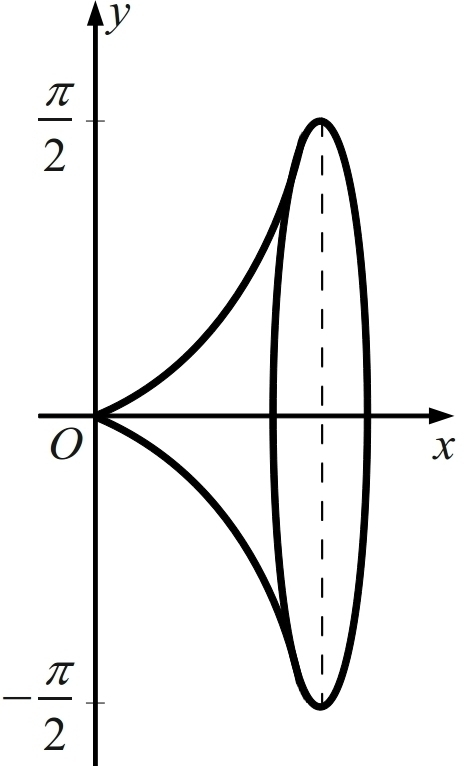
\includegraphics[height=5.11cm,bb=0 0 464 766]{1n.jpg}
   \caption{Тело вращения}\label{ris1}
\end{figure}

Пример вставки гиперссылки на запуск звукового файла 2.wma из папки <<media>>:
Послушаем \href{run:media/2.wma}{музыку}?

Пример вставки гиперссылки на запуск видео файла film.wmv из папки <<media>>:
\href{run:media/film.avi}{видеофильм}?

\section{Справочная информация}

Этот параграф можно назвать как угодно. Мы установим на первую страницу этого параграфа
метку \label{mybutton}, которая является <<мишенью>> Вашей кнопки на интерактивной панели
(описание процесса ее создания смотрите выше в комментариях).
\begin{enumerate}% Эта команда начинает список
\item Важная информация.
\item Очень важная информация.
\end{enumerate}% Эта команда завершает список

Если теперь скомпилировать <<Рабочий файл>>, то запустив электронный
учебник (файл UMK.pdf) и нажав на кнопку <<Ваша кнопка>> на интерактивной
панели, Вы попадете на эту страницу.

%--------------------------------------------------------------------------------------------

\section*{Вопросы и задания для самоконтроля}% Этот раздел будет состоять из вопросов
% и заданий для самоконтроля.
\addcontentsline{toc}{struct}{Вопросы и задания для самоконтроля}% Эта команда
% добавляет название раздела в раздел <<Содержание>>

Здесь можете привести список вопросов и заданий для самоконтроля:
\begin{enumerate}% Эта команда начинает список
\item Вопрос или задание.
\item Вопрос или задание.
\item Вопрос или задание.
\item Вопрос или задание.
\end{enumerate}% Эта команда завершает список

А можете подготовить с помощью программы IrenEditor (см. <<Руководство пользователю>>)
тестовое задание для самоконтроля, сохранить его в папку
<<test>>, назвав, например, lk1.exe, и создать на него метку с помощью
команды (см. <<Руководство пользователю>>): \href{run:test/lk1.exe}{Пройдем тестирование?}

%---------------------------------------------------------------------------------------------
\newpage% Эта команда задает разрыв страницы (начинает новую страницу).
\section*{ПРАКТИЧЕСКОЕ ЗАНЯТИЕ 1}% Эта команда начинает первое практическое занятие.
% Обратите внимание -- практические занятия придется нумеровать вручную.
\addcontentsline{toc}{chapter}{Практическое занятие 1 {\bf Тема занятия}} \vspace{-10pt}% Эти
% команды добавляют тему занятия в раздел <<Содержание>>
\begin{center}% Эта команда выравнивает текст по центру строки.
 {\bf% Эта команда делает шрифт полужирным
 Тема занятия}
\end{center}% Эта команда завершает <<центрирование>> текста.

{\bf Цель:} Сюда можно вписать цель практического занятия.
\\% Эта команда вставляет пустую строку.

Ваш текст.

%--------------------------------------------------------------------------------------------
\newpage% Эта команда начинает новую страницу
\section*{Задания для самостоятельного решения (выполнения)}% Эта команда начинает раздел с
% заданиями для самостоятельной работы
\addcontentsline{toc}{struct}{Задания для самостоятельного решения}% Эта команда добавляет
% название раздела в раздел <<Содержание>>

Ваш текст

\newpage% Эта команда задает новую страницу (разрыв страницы)

%--------------------------------------------------------------------------------------------

\newpage % Эта команда начинает новую страницу
\chapter{Тема лекции}% Эта команда начинает новую лекцию. В фигурных скобках нужно
% записать тему лекции. Эта тема лекции автоматически получит порядковый номер и
% автоматически добавится в раздел <<Содержание>>. Лекций можно создавать сколько угодно.
% Для создания новой лекции скопируйте и вставьте (или наберите с клавиатуры) команду
% \chapter{Тема лекции} в любую часть рабочего файла. Можете смело менять местами лекции --
% вся нумерация после очередной компиляции поменяется автоматически.

% При необходимости здесь можно разместить любой текст

\section{Название параграфа}% Эта команда начнет раздел, который будем далее условно называть
% параграф. В роли параграфа будет выступать структурная часть лекции (отдельный раздел,
% вопрос и т.п.). В фигурных скобках нужно вписать название параграфа. Параграф автоматически
% получит порядковый номер, который будет состоять из двух чисел, разделенных точкой.
% Первое число -- порядковый номер лекции, второе число -- порядковый номер параграфа в
% пределах лекции. Параграфов можно создавать сколько угодно. Для создания нового параграфа
% скопируйте и вставьте (или наберите с клавиатуры) команду \section{Название параграфа} в
% любую часть рабочего файла. Можете смело менять местами параграфы, переносить их из одной
% лекции  в другую -- вся нумерация после очередной компиляции поменяется автоматически.

% При необходимости здесь можно разместить любой текст

\subsection{Название подпараграфа}% Эта команда начинает подраздел, который далее будем
% условно называть подпараграфом. В фигурных скобках нужно вписать название подпараграфа.
% Подпараграф автоматически получит порядковый номер, который будет состоять из трех
% чисел, разделенных точками. Первое число -- порядковый номер лекции, второе число --
% порядковый номер параграфа, третье число -- порядковый номер подпараграфа. Подпараграфов
% можно создавать сколько угодно. Для создания нового подпараграфа скопируйте и вставьте
% (или наберите с клавиатуры) команду \subsection{Название подпараграфа} в любую часть
% Рабочего файла. Можете смело менять подпараграфы местами, переносить их из одного
% параграфа в другой (даже другой параграф другой лекции) -- вся нумерация после очередной
% компиляции поменяется автоматически.



%--------------------------------------------------------------------------------------------

\section*{Вопросы и задания для самоконтроля}% Этот раздел будет состоять из вопросов
% и заданий для самоконтроля.
\addcontentsline{toc}{struct}{Вопросы и задания для самоконтроля}% Эта команда
% добавляет название раздела в раздел <<Содержание>>

Здесь можете привести список вопросов и заданий для самоконтроля:
\begin{enumerate}% Эта команда начинает список
\item Вопрос или задание.
\item Вопрос или задание.
\item Вопрос или задание.
\item Вопрос или задание.
\end{enumerate}% Эта команда завершает список

А можете подготовить с помощью программы IrenEditor (см. <<Руководство пользователю>>)
тестовое задание для самоконтроля, сохранить его в папку
<<test>>, назвав, например, lk1.exe, и создать на него метку с помощью
команды (см. <<Руководство пользователю>>): \href{run:test/lk1.exe}{Пройдем тестирование?}

%---------------------------------------------------------------------------------------------
\newpage% Эта команда задает разрыв страницы (начинает новую страницу).
\section*{ПРАКТИЧЕСКОЕ ЗАНЯТИЕ 2}% Эта команда начинает второе практическое занятие.
% Обратите внимание -- практические занятия придется нумеровать вручную.
\addcontentsline{toc}{chapter}{Практическое занятие 2 {\bf Тема занятия}} \vspace{-10pt}% Эти
% команды добавляют тему занятия в раздел <<Содержание>>
\begin{center}% Эта команда выравнивает текст по центру строки.
 {\bf% Эта команда делает шрифт полужирным
 Тема занятия}
\end{center}% Эта команда завершает <<центрирование>> текста.

{\bf Цель:} Сюда можно вписать цель практического занятия.
\\% Эта команда вставляет пустую строку.

Ваш текст.

%--------------------------------------------------------------------------------------------
\newpage% Эта команда начинает новую страницу
\section*{Задания для самостоятельного решения (выполнения)}% Эта команда начинает раздел с
% заданиями для самостоятельной работы
\addcontentsline{toc}{struct}{Задания для самостоятельного решения}% Эта команда добавляет
% название раздела в раздел <<Содержание>>

Ваш текст

%--------------------------------------------------------------------------------------------

\newpage% Эта команда задает новую страницу (разрыв страницы)


\normalsize\section*{Варианты заданий для индивидуальной работы}% Эта команда создает новый
% раздел, название которого записано в фигурных скобках.
\addcontentsline{toc}{struct}{Варианты заданий для индивидуальной работы} % Эта
% команда добавляет название данного раздела к разделу <<Содержание>>

\begin{center}
   \bf{Вариант 1}
\end{center}

Ваш текст.

\begin{center}
   \bf{Вариант 2}
\end{center}

Ваш текст.

\begin{center}
   \bf{Вариант 3}
\end{center}

Ваш текст.

%--------------------------------------------------------------------------------------------

\newpage% Эта команда задает новую страницу (разрыв страницы)
{\large \section*{Вопросы для подготовки к экзамену и (или) зачету}% Эта команда начинает
% новый раздел, название которого записано в фигурных скобках
\addcontentsline{toc}{struct}{Вопросы для подготовки к экзамену и (или) зачету}% Эта
% команда добавляет название данного раздела к разделу <<Содержание>>

\begin{enumerate}% Эта команда начинает нумерованный список вопросов
 \item Вопрос.
\item Вопрос.
\item Вопрос.
\item Вопрос.
\end{enumerate}% Эта команда завершает нумерованный список вопросов

%--------------------------------------------------------------------------------------------

\newpage% Эта команда задает новую страницу (разрыв страницы)

\addtocontents{toc}{\vspace{15pt}}% Эту команду лучше не менять
\section*{Литература}% Эта команда начинает новый раздел, содержащий список литературы
\addcontentsline{toc}{struct}{Литература}% Эта
% команда добавляет название данного раздела к разделу <<Содержание>>

\itemsep=0pt% Эту команду лучше не менять
\parsep=0pt% Эту команду лучше не менять
\leftmargin=0mm \itemindent=0mm \labelsep=2mm \labelwidth=6mm% Эту команду лучше не менять
\rightmargin=0mm% Эту команду лучше не менять

\begin{enumerate}% Эта команда начинает нумерованный список литературы. На каждый элемент
% списка выставляйте свою метку (с помощью команды \label{name}, где name -- имя метки),
% чтобы иметь возможность ссылаться в тексте на любой элемент списка (см. <<Руководство
% пользователю>>.

\item\label{r8} Львовский,~С.М. Набор и вёрстка в пакете~\LaTeX.~---
М., Космосинформ, 1994.

\item\label{r1} Кнут,~Д. Всё про \TeX.~--- Протвино, RD\TeX, 1993.

\end{enumerate}% Эта команда завершает нумерованный список литературы.

%----------------------------------------------------------------------------------------

\label{pages_total}% Это метка на последнюю страницу электронного учебника. Она нужна для
% корректной работы интерактивного учебника

\end{document}% Эта команда завершает рабочий (исходный) файл электронного учебника
